\begin{exercice}[Dépenses culturelles et de loisirs]
Voici un texte analysant l'évolution de certaines dépenses culturelles et de loisirs des Suisses au cours des vingt dernières années. \\[0.5em]
« \emph{Les Suisses ont plus de temps libre, ce qui explique que leurs dépenses pour les loisirs (cinéma, concerts) augmentent régulièrement. Les dépenses en multimédia ont explosé au début des années 90 et sont constantes depuis. Nombreux sont ceux qui consultent les informations sur Internet et se désintéressent de la lecture des journaux...}

\emph{De même, les ventes de disques ou pellicules photo sont en diminution constante (cette catégorie est à présent la moins importante), ce qui s'explique par le « boum » de la photo numérique ou du téléchargement musical. Après avoir diminué, les ventes de téléviseurs ont tendance à redémarrer, grâce à la baisse des prix des écrans plats.} » \\[0.5em]
Le tableau suivant correspond au commentaire ci‑dessus. Les données sont données en pour cent.
 \begin{center}
  \renewcommand*\tabularxcolumn[1]{>{\centering\arraybackslash}m{#1}}
  \begin{ttableau}{\linewidth}{4}
   \hline
   \rowcolor{A2} \textbf{Dépense} & \textbf{1990} & \textbf{2000} & \textbf{2007} \\\hline
   \cellcolor{A2} \textbf{1} & 14,7 & 10,8 & 11,5 \\\hline
   \cellcolor{A2} \textbf{2} & 1,9 & 7,7 & 7,8 \\\hline
   \cellcolor{A2} \textbf{3} & 5,9 & 5,5 & 3,5 \\\hline
   \cellcolor{A2} \textbf{4} & 14,1 & 16,4 & 18,2 \\\hline
   \cellcolor{A2} \textbf{5} & 20,2 & 15,8 & 13,4 \\\hline
  \end{ttableau}
 \end{center}
\begin{enumerate}
 \item Indique à quelle catégorie de dépenses correspond chaque ligne du tableau, parmi les suivantes :
 \begin{itemize}
  \item Spectacles, cinéma et voyage ;
  \item Informatique ;
  \item Presse, livres et papeterie ;
  \item TV, Hi‑fi, vidéo ;
  \item Disques, cassettes, pellicules photo.
  \end{itemize}
 \item Calcule le total de chaque colonne du tableau. Comment expliques‑tu tes résultats ?
 \end{enumerate}
\end{exercice}



%%%%%%%%%%%%%%%%%%%%%%%%%%%%%%%%%%%
%%%%%%%%%%%%%%%%%%%%%%%%%%%%%%%%%%%
%MiseEnPage
%%%%%%%%%%%%%%%%%%%%%%%%%%%%%%%%%%%
\columnbreak
%%%%%%%%%%%%%%%%%%%%%%%%%%%%%%%%%%%
%%%%%%%%%%%%%%%%%%%%%%%%%%%%%%%%%%%

\begin{exercice}[Énergies renouvelables : prévisions]
Le tableau suivant indique le nombre d'emplois prévus dans différents secteurs des énergies renouvelables (\textcolor{PartieGeometrie}{en milliers d’emplois}).

Source : \emph{Rapport MITRE (2003) commandité par la Commission Européenne.}
 \begin{center}
 \begin{tabularx}{1.03\linewidth}{|c|X|X|X|X|X|X|X|X|X|}
  \hline
   & \cellcolor{H1} \rotatebox{90}{Biomasse} & \cellcolor{H1} \rotatebox{90}{Biocarburants} & \cellcolor{H1} \rotatebox{90}{Éolien} & \cellcolor{H1} \rotatebox{90}{Biogaz} & \cellcolor{H1} \rotatebox{90}{Solaire Thermique} & \cellcolor{H1} \rotatebox{90}{Photovoltaïque} & \cellcolor{H1} \rotatebox{90}{Micro-hydraulique\phantom{.}} & \cellcolor{H1} \rotatebox{90}{Pompes à chaleur} & \cellcolor{H1} \rotatebox{90}{\textbf{Total}} \\\hline
  \cellcolor{C2} Emplois en 2004 & \rotatebox{90}{25} & \rotatebox{90}{4.2\phantom{.}} & \rotatebox{90}{2} & \rotatebox{90}{0.1} & \rotatebox{90}{1} & \rotatebox{90}{1} & \rotatebox{90}{2.4} & \rotatebox{90}{3.2} & \\\hline
  \cellcolor{C2} Emplois en 2010 & \rotatebox{90}{45} & \rotatebox{90}{20} & & \rotatebox{90}{2} & \rotatebox{90}{10.5} & \rotatebox{90}{3.5} & \rotatebox{90}{2.4} & \rotatebox{90}{10} & \rotatebox{90}{115.4} \\\hline
  \end{tabularx}
\end{center}
\begin{enumerate}
 \item Combien d'emplois prévoit ce rapport pour la filière éolienne en 2010 ?
 \item Est‑il vrai que le nombre d'emplois dans le secteur des pompes à chaleur aura quasiment triplé entre 2004 et 2010 ?
 \item Combien d'emplois auront été créés entre 2004 et 2010 si ces prévisions se confirment ?
 \end{enumerate}
\end{exercice}

%%%%%%%%%%%%%%%%%%%%%%%%%%%%%%%%%%%
%%%%%%%%%%%%%%%%%%%%%%%%%%%%%%%%%%%
%MiseEnPage
%%%%%%%%%%%%%%%%%%%%%%%%%%%%%%%%%%%
\newpage
%%%%%%%%%%%%%%%%%%%%%%%%%%%%%%%%%%%
%%%%%%%%%%%%%%%%%%%%%%%%%%%%%%%%%%%

\begin{exercice}[Ça chauffe !]
Afin de surveiller ses dépenses de chauffage cet hiver, M. Frigo a décidé de contrôler sa consommation de mazout. Les graphiques suivants représentent la quantité de fuel restant dans sa cuve, en fonction du temps. \\[1em]
\textbf{\textcolor{A2}{En fin d'année}}

M. Frigo a commencé ses relevés fin novembre :
\begin{center} 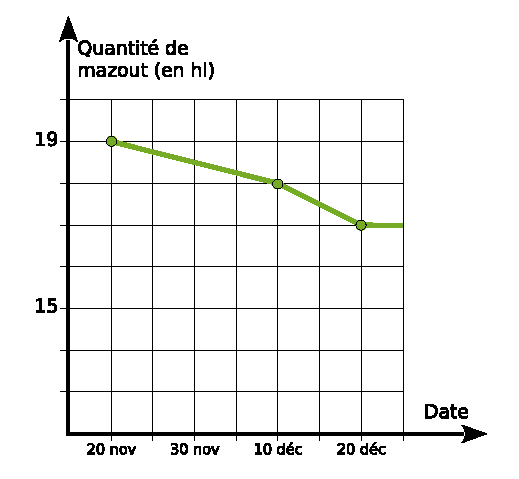
\includegraphics[width=8cm]{graph_frigo1} \end{center}

\begin{enumerate}
 \item Quelle quantité de mazout contenait sa cuve au 20 novembre ? 
 \item Quelle quantité de mazout a‑t‑il consommée du 20 novembre au 20 décembre ?
 \item Une vague de froid est survenue durant cette période \ldots Au vu du graphique, peux‑tu préciser quand ?
 \item Selon toi, M. Frigo a‑t‑il passé le jour de Noël à la maison ? Explique ta réponse. \\[1em]
 
 \textbf{\textcolor{A2}{Au début de l'année}}
 
\begin{center} 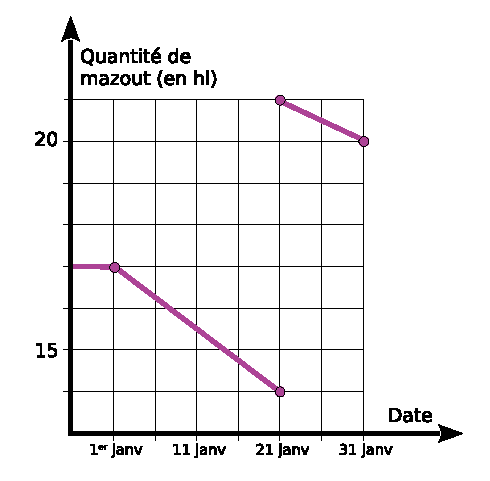
\includegraphics[width=8cm]{graph_frigo2} \end{center} 

 \item Quand M. Frigo a‑t‑il remis sa chaudière en route ?
 \item Que s'est‑il passé le 21 janvier ?
 \item Quelle quantité de mazout a‑t‑il consommée entre le 20 novembre et le 31 janvier ?
 \item Combien d'argent M. Frigo a‑t‑il dépensé durant cette période, sachant que le prix du litre de mazout était de 0,90 CHF ?
 \begin{center} 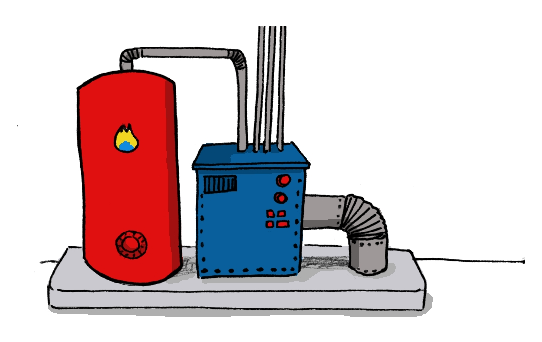
\includegraphics[width=4.5cm]{mazout} \end{center}
 \end{enumerate}
\end{exercice}



